\documentclass[12pt, titlepage]{article}

\usepackage{booktabs}
\usepackage{tabularx}
\usepackage{hyperref}
\hypersetup{
    colorlinks,
    citecolor=blue,
    filecolor=black,
    linkcolor=red,
    urlcolor=blue
}
\usepackage[round]{natbib}
\usepackage{graphicx}
\usepackage{longtable}

%% Comments

\usepackage{color}

\newif\ifcomments\commentstrue %displays comments
%\newif\ifcomments\commentsfalse %so that comments do not display

\ifcomments
\newcommand{\authornote}[3]{\textcolor{#1}{[#3 ---#2]}}
\newcommand{\todo}[1]{\textcolor{red}{[TODO: #1]}}
\else
\newcommand{\authornote}[3]{}
\newcommand{\todo}[1]{}
\fi

\newcommand{\wss}[1]{\authornote{blue}{SS}{#1}} 
\newcommand{\plt}[1]{\authornote{magenta}{TPLT}{#1}} %For explanation of the template
\newcommand{\an}[1]{\authornote{cyan}{Author}{#1}}

%% Common Parts

\newcommand{\progname}{MTOBridge} % PUT YOUR PROGRAM NAME HERE
\newcommand{\authname}{Team 15, Alpha Software Solutions
\\ Badawy, Adham
\\ Yazdinia, Pedram
\\ Jandric, David
\\ Vakili, Farzad
\\ Vezina, Victor
\\ Chiu, Darren} % AUTHOR NAMES                  

\usepackage{hyperref}
    \hypersetup{colorlinks=true, linkcolor=blue, citecolor=blue, filecolor=blue,
                urlcolor=blue, unicode=false}
    \urlstyle{same}


\graphicspath{{images/}}

\begin{document}

\title{Project Title: System Verification and Validation Plan for \progname{}} 
\author{\authname}
\date{\today}
	
\maketitle

\pagenumbering{roman}

\section{Revision History}

\begin{tabularx}{\textwidth}{p{3cm}p{2cm}X}
\toprule {\bf Date} & {\bf Version} & {\bf Notes}\\
\midrule
October 30 & Darren & Non-Functional System Tests\\
November 1 & Pedram & Functional System Tests\\
November 1 & Victor & Unit Tests Intro\\
November 1 & Victor & Non-Functional System Tests\\
\bottomrule
\end{tabularx}

\newpage

\tableofcontents

\listoftables
\wss{Remove this section if it isn't needed}

\listoffigures
\wss{Remove this section if it isn't needed}

\newpage

\section{Symbols, Abbreviations and Acronyms}

\renewcommand{\arraystretch}{1.2}
\begin{tabular}{l l} 
  \toprule		
  \textbf{symbol} & \textbf{description}\\
  \midrule 
  T & Test\\
  \bottomrule
\end{tabular}\\

\wss{symbols, abbreviations or acronyms -- you can simply reference the SRS
  \citep{SRS} tables, if appropriate}

\newpage

\pagenumbering{arabic}

This document ... \wss{provide an introductory blurb and roadmap of the
  Verification and Validation plan}

\section{General Information}

\subsection{Summary}

\wss{Say what software is being tested.  Give its name and a brief overview of
  its general functions.}

\subsection{Objectives}

\wss{State what is intended to be accomplished.  The objective will be around
  the qualities that are most important for your project.  You might have
  something like: ``build confidence in the software correctness,''
  ``demonstrate adequate usability.'' etc.  You won't list all of the qualities,
  just those that are most important.}

\subsection{Relevant Documentation}

\wss{Reference relevant documentation.  This will definitely include your SRS
  and your other project documents (MG, MIS, etc).  You can include these even
  before they are written, since by the time the project is done, they will be
  written.}

\citet{SRS}

\section{Plan}

\wss{Introduce this section.   You can provide a roadmap of the sections to
  come.}

\subsection{Verification and Validation Team}

\wss{You, your classmates and the course instructor.  Maybe your supervisor.
  You shoud do more than list names.  You should say what each person's role is
  for the project.  A table is a good way to summarize this information.}

\subsection{SRS Verification Plan}

\wss{List any approaches you intend to use for SRS verification.  This may just
  be ad hoc feedback from reviewers, like your classmates, or you may have
  something more rigorous/systematic in mind..}

\wss{Remember you have an SRS checklist}

\subsection{Design Verification Plan}

\wss{Plans for design verification}

\wss{The review will include reviews by your classmates}

\wss{Remember you have MG and MIS checklists}

\subsection{Implementation Verification Plan}

\wss{You should at least point to the tests listed in this document and the unit
  testing plan.}

\wss{In this section you would also give any details of any plans for static verification of
  the implementation.  Potential techniques include code walkthroughs, code
  inspection, static analyzers, etc.}

\subsection{Automated Testing and Verification Tools}

\wss{What tools are you using for automated testing.  Likely a unit testing
  framework and maybe a profiling tool, like ValGrind.  Other possible tools
  include a static analyzer, make, continuous integration tools, test coverage
  tools, etc.  Explain your plans for summarizing code coverage metrics.
  Linters are another important class of tools.  For the programming language
  you select, you should look at the available linters.  There may also be tools
  that verify that coding standards have been respected, like flake9 for
  Python.}

\wss{The details of this section will likely evolve as you get closer to the
  implementation.}

\subsection{Software Validation Plan}

\wss{If there is any external data that can be used for validation, you should
  point to it here.  If there are no plans for validation, you should state that
  here.}

\section{System Test Description}
	
\subsection{Tests for Functional Requirements}

\wss{Subsets of the tests may be in related, so this section is divided into
  different areas.  If there are no identifiable subsets for the tests, this
  level of document structure can be removed.}

\wss{Include a blurb here to explain why the subsections below
  cover the requirements.  References to the SRS would be good.}

\subsubsection{Area of Testing1}

\wss{It would be nice to have a blurb here to explain why the subsections below
  cover the requirements.  References to the SRS would be good.  If a section
  covers tests for input constraints, you should reference the data constraints
  table in the SRS.}
		

\begin{enumerate}

\item{test-id1\\}

Control: Automatic
					
Initial State: 
					
Input: 
					
Output: \wss{The expected result for the given inputs}

Test Case Derivation: \wss{Justify the expected value given in the Output field}
					
How test will be performed: 
					
\item{test-id2\\}

Control: Automatic
					
Initial State: 
					
Input: 
					
Output: \wss{The expected result for the given inputs}

Test Case Derivation: \wss{Justify the expected value given in the Output field}

How test will be performed: 

\end{enumerate}

\subsubsection{File Manager}

\begin{enumerate}

\item{UTFR-2.1\\}

Control: Automatic
					
Initial State: None
					
Input: File location path
					
Output: New MTOBridge instance initialized with the given data instead of the default 

Test Case Derivation: Config file contains data that were previously inputted by a user, so to the load the data we have to restart the process 
					
How test will be performed: The test involves instantiating an MTOBridge process with the saved data and then running our logic checks to validate the saved input.
					
\item{UTFR-2.2\\}

Control: Automatic
					
Initial State: None
					
Input: File location path 
					
Output: Boolean variable indicating True or False 

Test Case Derivation: Require a method to check for the integrity of the saved configurations as the data can be faulty or incomplete

How test will be performed: The test is performed by validating the completeness and metadata of the file to make sure the file hasn't been corrupted hence preventing an instance construct call with faulty data.

\end{enumerate}

\subsubsection{Solver Setup}

\begin{enumerate}

\item{UTFR-3.1\\}

Control: Automatic
					
Initial State: None
					
Input: text input to indicate the desired solver 
					
Output: Calculation results based on the selected solver

Test Case Derivation: The current logic allows for calculation of the demand at different areas called concerened sections. These can show the forces for both a single section as well as the entire bridge. 

How test will be performed: The test involves running a series of pre-determined calculation using both solvers and then comparing with the auotmaic output selecting one solver at a time. 
					

\end{enumerate}

\subsubsection{Bridge Config}

\begin{enumerate}

\item{UTFR-4.1\\}

Control: Automatic
					
Initial State: None
					
Input: text input to indicate the desired section 
					
Output: Calculation results based on the selected section

Test Case Derivation: The current logic allows for calculation of the demand at different areas called concerened sections. These can show the forces for both a single section as well as the entire bridge. 

How test will be performed: Once the section is selected, the test is performed by executing different types of platoon and bridge characteristic to derive actual results. These results are validated and compared to the exepected results calculated through the engine only. 
					
\item{UTFR-4.2\\}

Control: Automatic
					
Initial State: None
					
Input: text input to indicate the discretization length 
					
Output: Calculation results based on the defined length

Test Case Derivation: In order to use the second solver, the system requires information on the number of equally spaced parts of the bridge. 

How test will be performed: Using an array of discretization lengths, we can take advantage of the engine's efficiency to calculate the maximum demand force in different context and compare with our own expected results. 

\end{enumerate}


\subsubsection{Calculation Parameters}

\begin{enumerate}

\item{UTFR-5.1\\}

Control: Automatic
					
Initial State: None
					
Input: text input to indicate the desired force type  
					
Output: Calculation results based on the selected parameters 

Test Case Derivation: The current implmentation of the engine allows for calculation across shear, torsion and flexural resistance

How test will be performed: The test entails creating a series of bridge types with different truck platoons that can be tested for all force types such as shear, torsion and flexural. Each data test is manually fed into the engine to output an expected output. 
					
\item{UTFR-5.2\\}

Control: Automatic
					
Initial State: None
					
Input: text input to indicate the desired moment  
					 
Output: Calculation results based on the selected parameters 

Test Case Derivation: The current implmentation of the engine allows for calculation using postivie and negative moment 

How test will be performed: The test will be performed by using our pool of pre-determined bridge and truck platoon configs to test for both positive and negative moment given a certain force type. 

\end{enumerate}

\subsubsection{Result Visualizer}

\begin{enumerate}

\item{UTFR-6.1\\}

Control: Automatic
				
Initial State: None
					
Input: calculations based on the concerened section 
					
Output: Animation and visualiation highlighting the resulting properties on the specified bridge and load 

Test Case Derivation: As one of the main purposes of the program, the visualization will be interactable to show various views

How test will be performed: Relying on the pre-determined and validated data, we will graph the visulizations of each through the system as well as manually through the data produced by the engine. We can then compare the the expected and actual result across all available views. 
					
\item{UTFR-6.2\\}

Control: Automatic
					
Initial State: None
					
Input: calculations based on the discretization length 
					
Output:  Animation and visualiation highlighting the resulting properties on the specified bridge and load 

Test Case Derivation: As one of the main purposes of the program, the visualization will be interactable to show various views

How test will be performed: Relying on the pre-determined and validated data, we will graph the visulizations of each through the system as well as manually through the data produced by the engine. We can then compare the the expected and actual result across all available views. 

\end{enumerate}

\subsubsection{Exectution Flow Logging}

\begin{enumerate}

\item{UTFR-7.1\\}

Control: Automatic
					
Initial State: None
					
Input: text input to indicate logging flags 
					
Output: text output, "logs"

Test Case Derivation: With the engine built in another framework, its important to log every state change throughout the calculations as triggered by the system

How test will be performed: While running multiple calculations, the system is asked to comprehensively log the flow in the engine. The system will be interrupted at times to test the robustness as well. The resulting logs should be clearly highlighting the steps taken including any errors or warnings.
					

\end{enumerate}


\subsection{Tests for Nonfunctional Requirements}

\wss{The nonfunctional requirements for accuracy will likely just reference the
  appropriate functional tests from above.  The test cases should mention
  reporting the relative error for these tests.}

\wss{Tests related to usability could include conducting a usability test and
  survey.}

\subsubsection{Look and Feel Requirements}
		
\paragraph{Graphics Informative Value Test}

\begin{enumerate}

\item{NFR1.ST1\\}

Initial State: Bridge UI mockups containing graphic elements will be prepared

Type: Manual, Static

How test will be performed: Civil engineers will be presented with mockups and expected to identify what the graphic elements represent with at least 90\% accuracy. Refer to Figure \ref{fig:ui-mockup} for example UI mockup.

\end{enumerate}

\subsubsection{Usability and Humanity Requirements}
		
\paragraph{Intuitiveness Test}

\begin{enumerate}

\item{NFR2.ST1\\}

Initial State: Application is opened with no past data

Type: Manual, Dynamic

Input/Condition: User inputs

Output/Results: Bridge analysis within 5 minutes of introduction

How test will be performed: Civil engineer will be asked to provide inputs

\end{enumerate}
		
\paragraph{Display Resolution Test}

\begin{enumerate}

\item{NFR3.ST1\\}

Initial State: Application is opened

Type: Manual, Dynamic

Input/Condition: Application is running on a computer with 1280x720 display

Output/Results: All buttons and animation window remain visible and accessible

\item{NFR3.ST2\\}

Repeat test NFR.ST3 for 1366x768 display

\item{NFR3.ST3\\}

Repeat test NFR.ST3 for 1920x1080 display

\item{NFR3.ST4\\}

Repeat test NFR.ST3 for 2560x1440 display

\item{NFR3.ST5\\}

Repeat test NFR.ST3 for 3840x2160 display

\end{enumerate}

\paragraph{Text Resizing Test}

\begin{enumerate}

\item{NFR4.ST1\\}

Initial State: Application is opened with no past data

Type: Manual, Dynamic

Input/Condition: Font size setting is changed to display as 8pt

Output/Results: All buttons and animation window remain visible and accessible

How test will be performed: 

\item{NFR4.ST2\\}

Repeat test NFR.ST8 with font size 16pt

\item{NFR4.ST3\\}

Repeat test NFR.ST8 with font size 24pt

\item{NFR4.ST4\\}

Repeat test NFR.ST8 with font size 32pt

\end{enumerate}

\paragraph{Ease of Installation Test}

\begin{enumerate}

\item{NFR5.ST1\\}

Initial State: Application is not installed

Type: Manual

Input/Condition: Application is downloaded and installed

Output/Results: Application is ready to use within 30 minutes

How test will be performed: By civil engineer

\end{enumerate}

\paragraph{Consistent UI Test}

\begin{enumerate}

\item{NFR6.ST1\\}

Initial State: Visually similar UI elements are grouped into categories by developers

Type: Manual, Static

Input/Condition: Civil engineer asked to associate UI elements with their respective categories

Output/Results: Civil engineer sorts at least 90\% of UI elements into their predefined categories

\end{enumerate}

\subsubsection{Performance Requirements}

\paragraph{UI Speed Test}

\begin{enumerate}

\item{NFR10.ST1\\}

Initial State: Application is opened with no past data

Type: Manual, Dynamic

Input/Condition: Application used to generate a small bridge analysis whose total execution time is at most \textcolor{red}{X} seconds

Output/Results: Total execution time will not exceed underlying MATLAB script's execution time by 10\%

\item{NFR10.ST2\\}

Initial State: Application is opened with no past data

Type: Manual, Dynamic

Input/Condition: Application used to generate a large bridge analysis whose total execution time is at least \textcolor{red}{Y} seconds

Output/Results: Total execution time will not exceed underlying MATLAB script's execution time by 10\%

\end{enumerate}

\subsubsection{Operational and Environmental Requirements}
		
\paragraph{User Computer Test}

\begin{enumerate}

\item{NFR12.ST1\\}

Initial State: Application is opened on expected users' computer

Type: Manual, Dynamic

Input/Condition: Application used to generate a small bridge analysis

Output/Results: Time needed on user computer will not exceed time needed on developer computers by 10\%(?)

How test will be performed: The bridge analysis configuration will be one whose total execution time is at most \textcolor{red}{X} seconds on developer computers

\item{NFR12.ST2\\}

Initial State: Application is opened on expected users' computer

Type: Manual, Dynamic

Input/Condition: Application used to generate a large bridge analysis

Output/Results: Time needed on user computer will not exceed time needed on developer computers by 10\%(?)

How test will be performed: The bridge analysis configuration will be one whose total execution time is at least \textcolor{red}{Y} seconds on developer computers

\end{enumerate}

\subsubsection{Maintainability and Support Requirements}
		
\paragraph{Ease of Maintenance Test}

\begin{enumerate}

\item{NFR13.ST1\\}

Type: Automatic, Static

Input/Condition: Measure code file length in lines

Output/Results: At least 75\% of files will contain 750 lines of code or less

How test will be performed: 

\item{NFR13.ST2\\}

Type: Automatic, Static

Input/Condition: Measure method length in lines

Output/Results: At least 75\% of methods will contain 75 lines of code or less

How test will be performed: 

\item{NFR13.ST3\\}

Type: Automatic, Static

Input/Condition: Measure length of code lines

Output/Results: At least 75\% of lines will contain \textcolor{red}{\bf 120} characters or less

How test will be performed: 

\item{NFR13.ST4\\}

Type: Automatic, Static

Input/Condition: Measure nesting depth of methods

Output/Results: At least 75\% of methods will have a maximum nesting depth of 5 or less

How test will be performed: 

\end{enumerate}

\subsection{Traceability Between Test Cases and Requirements}

\begin{longtable}{|p{0.2\textwidth} | p{0.8\textwidth}|}
  \caption{System Test Traceability}
  \label{TblSTTraceability}\\
  \hline
  \textbf{Requirement} & \textbf{System Tests}\\
  \hline
  NFR1 & NFR1.ST1\\
  \hline
  NFR2 & NFR2.ST1\\
  \hline
  NFR3 & NFR3.ST1, NFR3.ST2, NFR3.ST3, NFR3.ST4, NFR3.ST5\\
  \hline
  NFR4 & NFR4.ST1, NFR4.ST2, NFR4.ST3, NFR4.ST4\\
  \hline
  NFR5 & NFR5.ST1\\
  \hline
  NFR6 & NFR6.ST1\\
  \hline
  NFR7 & \\
  \hline
  NFR8 & \\
  \hline
  NFR9 & \\
  \hline
  NFR10 & NFR10.ST1, NFR10.ST2\\
  \hline
  NFR11 & \\
  \hline
  NFR12 & NFR12.ST1, NFR12.ST2\\
  \hline
  NFR13 & NFR13.ST1, NFR13.ST2, NFR13.ST3, NFR13.ST4\\
  \hline
  NFR14 & \\
  \hline
  NFR15 & \\
  \hline
\end{longtable}


\section{Unit Test Description}

As outlined in our \href{https://github.com/agentvv/MTOBridge/blob/main/docs/DevelopmentPlan/DevelopmentPlan.pdf}{Development Plan}, we will be using Qt Test and Google Test to conduct our unit testing. These testing frameworks will allow us to create and run unit tests quickly and easily.

\subsection{Unit Testing Scope}

\wss{What modules are outside of the scope.  If there are modules that are
  developed by someone else, then you would say here if you aren't planning on
  verifying them.  There may also be modules that are part of your software, but
  have a lower priority for verification than others.  If this is the case,
  explain your rationale for the ranking of module importance.}

\subsection{Tests for Functional Requirements}

\wss{Most of the verification will be through automated unit testing.  If
  appropriate specific modules can be verified by a non-testing based
  technique.  That can also be documented in this section.}

\subsubsection{Module 1}

\wss{Include a blurb here to explain why the subsections below cover the module.
  References to the MIS would be good.  You will want tests from a black box
  perspective and from a white box perspective.  Explain to the reader how the
  tests were selected.}

\begin{enumerate}

\item{test-id1\\}

Type: \wss{Functional, Dynamic, Manual, Automatic, Static etc. Most will
  be automatic}
					
Initial State: 
					
Input: 
					
Output: \wss{The expected result for the given inputs}

Test Case Derivation: \wss{Justify the expected value given in the Output field}

How test will be performed: 
					
\item{test-id2\\}

Type: \wss{Functional, Dynamic, Manual, Automatic, Static etc. Most will
  be automatic}
					
Initial State: 
					
Input: 
					
Output: \wss{The expected result for the given inputs}

Test Case Derivation: \wss{Justify the expected value given in the Output field}

How test will be performed: 

\item{...\\}
    
\end{enumerate}

\subsubsection{Module 2}

...

\subsection{Tests for Nonfunctional Requirements}

\wss{If there is a module that needs to be independently assessed for
  performance, those test cases can go here.  In some projects, planning for
  nonfunctional tests of units will not be that relevant.}

\wss{These tests may involve collecting performance data from previously
  mentioned functional tests.}

\subsubsection{Module ?}
		
\begin{enumerate}

\item{test-id1\\}

Type: \wss{Functional, Dynamic, Manual, Automatic, Static etc. Most will
  be automatic}
					
Initial State: 
					
Input/Condition: 
					
Output/Result: 
					
How test will be performed: 
					
\item{test-id2\\}

Type: Functional, Dynamic, Manual, Static etc.
					
Initial State: 
					
Input: 
					
Output: 
					
How test will be performed: 

\end{enumerate}

\subsubsection{Module ?}

...

\subsection{Traceability Between Test Cases and Modules}

\wss{Provide evidence that all of the modules have been considered.}
				
\bibliographystyle{plainnat}

\bibliography{../../refs/References}

\newpage

\section{Appendix}

This is where you can place additional information.

\begin{figure}[]
  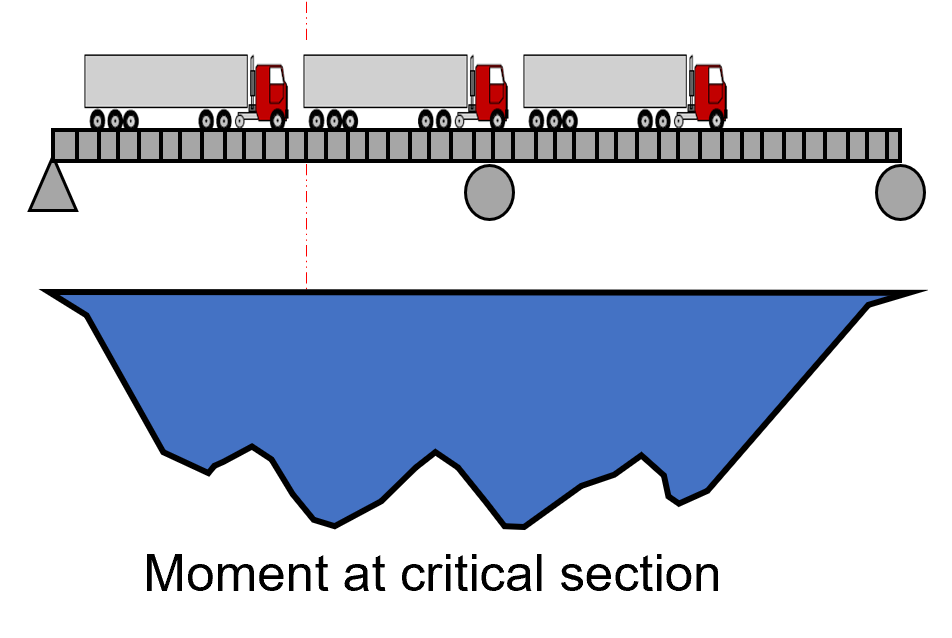
\includegraphics[width=\linewidth]{UI.png}
  \caption{UI mockup}
  \label {fig:ui-mockup}
\end{figure}

\subsection{Symbolic Parameters}

The definition of the test cases will call for SYMBOLIC\_CONSTANTS.
Their values are defined in this section for easy maintenance.

\subsection{Usability Survey Questions?}

\wss{This is a section that would be appropriate for some projects.}

\newpage{}
\section*{Appendix --- Reflection}

The information in this section will be used to evaluate the team members on the
graduate attribute of Lifelong Learning.  Please answer the following questions:

\begin{enumerate}
  \item What knowledge and skills will the team collectively need to acquire to
  successfully complete the verification and validation of your project?
  Examples of possible knowledge and skills include dynamic testing knowledge,
  static testing knowledge, specific tool usage etc.  You should look to
  identify at least one item for each team member.
  \item For each of the knowledge areas and skills identified in the previous
  question, what are at least two approaches to acquiring the knowledge or
  mastering the skill?  Of the identified approaches, which will each team
  member pursue, and why did they make this choice?
\end{enumerate}

\end{document}